\documentclass[11pt]{beamer}

\usepackage[T1]{fontenc}
\usepackage[utf8x]{inputenc}

%% Fonts
\usepackage{multicol}
\usepackage{mathabx}
\usepackage[scaled]{helvet}
\usepackage{lmodern}
\usepackage{eulervm}
\usefonttheme[onlymath]{serif}
\usefonttheme{professionalfonts}
\usefonttheme{structurebold}

\usepackage{hyperref}

\usepackage{bm}
\usepackage{pgf}
\usepackage{natbib}

%% Color & Theme
\usetheme{AnnArbor}

\setbeamerfont{title}{size=\large}
\setbeamerfont{frametitle}{size=\large}

\definecolor{SUblue}{RGB}{0,0,180}
% \usecolortheme[RGB={0,0,180}]{structure}
% \usetheme{Boadilla}
\setbeamertemplate{navigation symbols}{}
% \setbeamertemplate{itemize items}[circle]
% \setbeamertemplate{enumerate items}[circle]
% \setbeamerfont{title}{size=\large}
% \setbeamerfont{frametitle}{size=\large}
\setbeamerfont{framesubtitle}{size=\large,shape =$\color{violet}{\looparrowdownright}~$}
% \setbeamercolor{title}{fg=white, bg= SUblue!75!green}
% \setbeamercolor{framesubtitle}{fg=violet}
% \setlength{\leftmargini}{5pt}


% \hypersetup{colorlinks=true, linkcolor=blue}

\title[Bayesian Conditional Densities]{Bayesian Modeling of
  Conditional Densities}

\subtitle{---Presentation on the Cramér Society 2014 Annual Meeting}

\author[Feng Li]{\textbf{Feng Li}\\\texttt{ <feng.li@cufe.edu.cn>}}

\institute[Stat\&Math, CUFE]{\footnotesize{\textbf{BEFORE:\\ Department
      of Statistics, Stockholm University\\\vspace{1cm}NOW:\\School of
      Statistics and Mathematics\\ Central University of Finance and
      Economics, Beijing\\}}} \date{}


%%%%%%%%%%%%%%%%%%%%%%%%%%%%%%%%%%%%%%%%%%%%%%%%%%%%%%%%%%%%%%%%%%%%%%%%%%%%%%%
\begin{document}


%% Title page
\begin{frame}[plain]
  \titlepage
  % \tiny{Revision: \today}
\end{frame}


\begin{frame}[plain]
  % \titlepage
  \begin{figure}
    \centering
    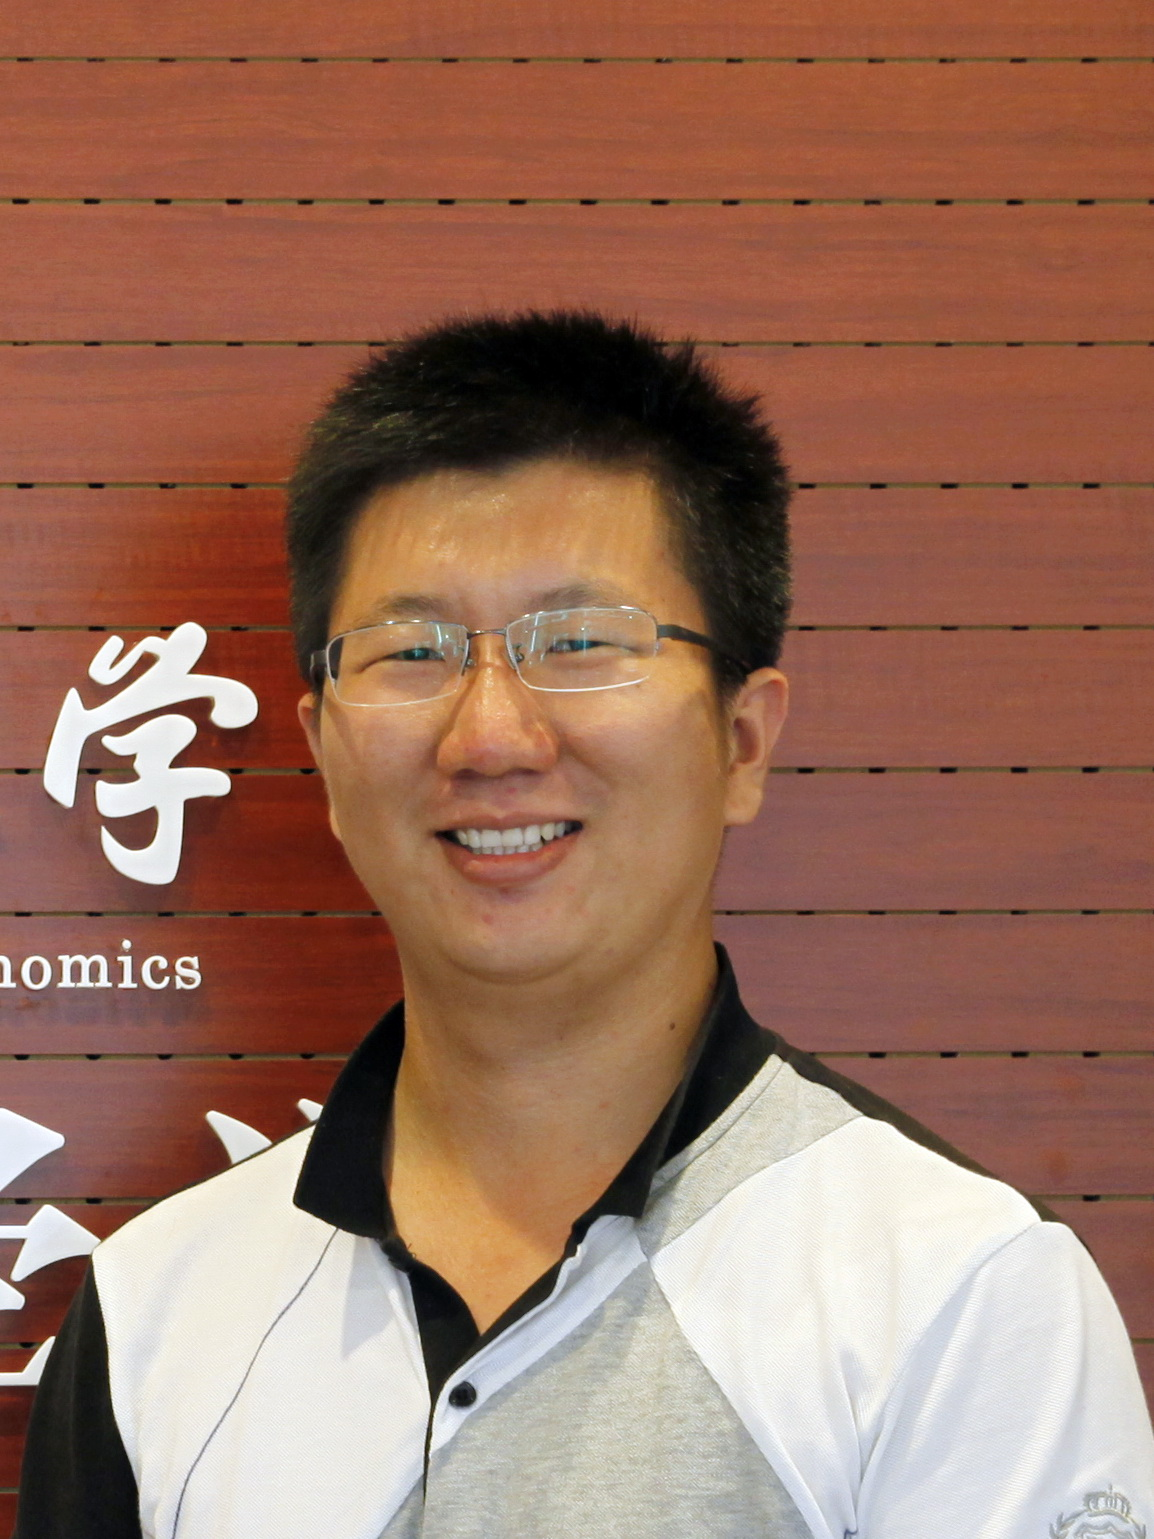
\includegraphics[height=0.9\textheight]{FengLi}
    \caption{This is how I look now.}
  \end{figure}
  % \tiny{Revision: \today}
\end{frame}


%% Outline page
\section*{Outline}
\begin{frame}
  \frametitle{Outline}
  \tableofcontents
\end{frame}
%%%%%%%%%%%%%%%%%%%%%%%%%%%%%%%%%%%%%%%%%%%%%%%%%%%%%%%%%%%%%%%%%%%%%%



\section{Conditional density models}
\begin{frame}
  % \frametitle{Knowing the elephant}
  \frametitle{The trend of statistical modeling}

  \begin{itemize}
  \item In the 1950s, linear regression model  was considered as very advanced
    which is now the standard course content for university students.
  \item The data are much more complicated nowadays we meet.
    \begin{itemize}
    \item Numerical, categorical, texts, brain image...
    \item Data volume from a few observations to millions by millions.
    \item Very high-dimensional data are not rare anymore.
    \end{itemize}
  \end{itemize}
\end{frame}


\begin{frame}
  \frametitle{Density estimation}
  \begin{itemize}
  \item \textbf{Density estimation} is the procedure of estimating an unknown density
    $p(y)$ from observed data

  \item Histogram, kernel methods, splines, wavelets are all density estimation
    methods.

  \item \textbf{Mixture models} \citep{jiang1999approximation} have become a popular alternative approach,
    \[
    p(y|\theta)=\sum\limits _{k=1}^{K}\omega_{k}p_{k}(y|\theta_{k}),
    \]
    where $\sum\nolimits _{k=1}^{K}\omega_{k}=1$ for non-negative mixture
    \textbf{weights} $\omega_{k}$ and $p_{k}(x|\theta_{k})$ are the \textbf{
      component densities}.

  \item If $K=\infty$, it is called an \textbf{infinite mixture} \citep{escobar1994estimating}, the
    \textbf{Dirichlet process mixture} being the most prominent example.

  \item Mixture densities can be used to capture data characteristics such as
    multi-modality, fat tails.

  \end{itemize}

\end{frame}


\begin{frame}
  \begin{figure}
    \centering
    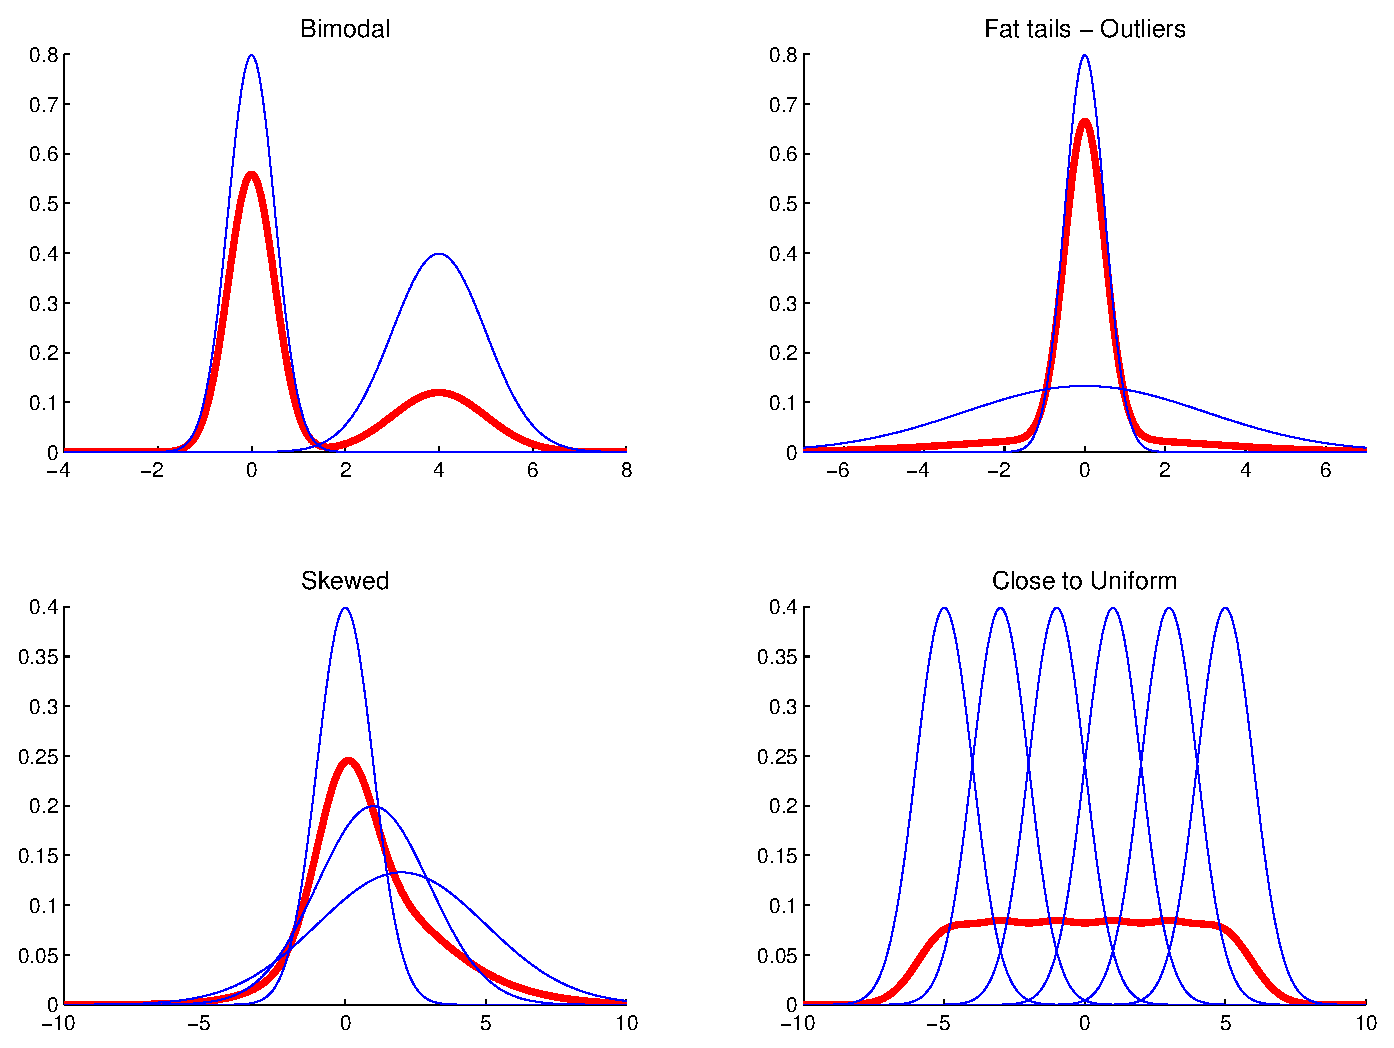
\includegraphics[width=10cm]{MixtureOfNormals2}\caption{Using mixture of normal
      densities (thin lines) to mimic a flexible density (bold line).}
    \label{fig: mix-norm}
  \end{figure}
\end{frame}


\begin{frame}
  \frametitle{One-dimensional conditional density estimation with mixtures}

  \begin{itemize}
  \item The \textbf{conditional density estimation} concentrates on modeling the
    relationship between a response $y$ and set of covariates $x$ through a
    conditional density function $p(y|x)$

  \item Mixtures of conditional densities is the obvious extension of mixture
    models to the conditional density estimation problem:
    \[
    p(y|x)=\sum\nolimits _{k=1}^{K}\omega_{k}p_{k}(y|x)
    \]
    where $p_{i}(y|x)$ is the conditional density in $i$:th mixture component.

  \item A \textbf{smooth mixture} is a finite mixture density with weights that
    are smooth functions of the covariates
    \[
    \omega_{k}(x)=\frac{\exp(x'\gamma_{k})}{\sum_{i=1}^{K}\exp(x'\gamma_{i})}.
    \]
  \end{itemize}

\end{frame}



\begin{frame}
  \frametitle{One-dimensional conditional density estimation with splines}

  \begin{itemize}
  \item In conditional density estimation, an important focus is modeling
    the regression mean $E(y|x)$.

  \item A \textbf{spline} is a popular approach for nonlinear regression that
    models the mean as a linear combination of a set of nonlinear basis
    functions of the original regressors \citep{holmes2003generalized},
    \[
    y=f(x)+\epsilon=x'\beta+\sum\nolimits _{i=1}^{k}x(\xi_{i})'\beta_{i}+\epsilon
    \]

  \end{itemize}
\end{frame}


\begin{frame}
  \frametitle{Multivariate density estimation with copulas}
  \begin{itemize}
  \item The \textbf{multivariate density estimation} and conditional density estimation
    are analogues of their univariate cases except that the densities
    $p(\bm{Y})$ and $p(\bm{Y}|\bm{X})$ are multivariate.

  \item In addition to the methods mentioned above, a \textbf{copula function}
    separates the multivariate dependence from its marginal functions, and it
    is possible to use both continuous and discrete marginal models.

  \item Let $F(y_{1},...,y_{M})$ be a multi-dimensional distribution function
    with marginal distribution functions
    $F_{1}(y_{1}),\cdots,F_{M}(y_{M})$. Then there exists a copula function $C$
    \citep{sklar1959fonctions} such
    that
    \[
    \begin{split}
&F(y_{1},...,y_{M})=  C(F_{1}(y_{1}),...,F_{M}(y_{M}))\\
      &=  C\left(\int_{-\infty}^{y_{1}}f_{1}(z_{1})dz_{1},...,\int_{-\infty}^{y_{M}}f_{M}(z_{M})dz_{M}\right)=C(u_{1},...,u_{M})
    \end{split}
    \]
  \end{itemize}

\end{frame}


\begin{frame}
  \frametitle{Multivariate density estimation with copulas}

  \begin{itemize}
  \item The \textbf{Kendall's $\tau$ correlation} between two marginal
    densities can be measured by Kendall's $\tau$
    \[
    \tau=4\int\int F(y_{1},y_{2})\mathrm{d}F(y_{1},y_{2})-1=4\int\int
    C(u_{1},u_{2})\mathrm{d}C(u_{1},u_{2})-1.
    \]

  \item \textbf{Tail-dependence} measures the extent to which
    several variables simultaneously take on extreme values
    \[
    \begin{split}\lambda_{L}= & \lim\limits _{u\to0^{+}}Pr(X_{1}<F_{1}^{-1}(u)|X_{2}<F_{2}^{-1}(u))=\lim\limits _{u\to0^{+}}\frac{C(u,u)}{u},\\
      \lambda_{U}= & \lim\limits _{u\to1^{-}}Pr(X_{1}>F_{1}^{-1}(u)|X_{2}>F_{2}^{-1}(u))=\lim\limits _{u\to1^{-}}\frac{1-C(u,u)}{1-u}.
    \end{split}
    \]

  \item Modeling tail-dependence is an very important topic in econometrics
    \citep{joe1997multivariate} \citep{patton2012review}.

  \end{itemize}



\end{frame}





\begin{frame}
  \frametitle{The Bayesian approach for modeling density features}
  \framesubtitle{A feature of a density}

  \begin{itemize}
  \item We use the word \textbf{feature} to describe a characteristic of a
    density.

  \item In GLM or splines, $\mu = \eta (X\beta)$ is the feature that describes the \textbf{mean}.

  \item In mixtures contents, the \textbf{mean}, \textbf{variance},
    \textbf{skewness} and \textbf{kurtosis} are features of each component
    density.

  \item In copula modeling, the \textbf{tail-dependence} and
    \textbf{correlation} are two features of interest.

  \item We allow each of the features are connected to covariates as
    \begin{align*}
        \mu & =  \beta_{\mu0}+x_{t}'\beta_{\mu} &
        \ln\phi & =  \beta_{\phi0}+x_{t}'\beta_{\phi} \\
        \ln\lambda & =  \beta_{\lambda0}+x_{t}'\beta_{\lambda} &
        \ln\nu & = \beta_{\nu0}+x_{t}'\beta_{\nu}\\
        \lambda_L & = \varphi_{\lambda}^{-1}(X\beta_\lambda) &
        \tau &= \varphi_{\tau}^{-1}(X\beta_\tau).
    \end{align*}

  \item This approach allows the feature to be dynamic and interpretable
    friendly.

  \item We only need to sample the posterior of $p(\beta|Data)$.

  \end{itemize}

\end{frame}

\section{Bayesian approach for modeling conditional density}


\begin{frame}
  \frametitle{The Bayesian approach for modeling density features}
  \framesubtitle{The efficient MCMC scheme}

  \begin{itemize}

  \item The model settings are very complicated now.

  \item Sampling the posterior requires an efficient MCMC method.

  \item We update all the parameters jointly by using
    Metropolis-Hastings within Gibbs.
  \item The proposal density for each parameter vector $\beta$ is a multivariate \emph{t}-density with  $df>2$,
    \[
    \bm{\beta}_{p} |\bm{\beta}_{c}\sim\bm{MVT}\left[\bm{\hat{\beta}},~\left.-\left(\frac{\partial^{2}\ln
            p(\bm{\beta}|\bm{Y})}{\partial\bm{\beta}\partial\bm{\beta}^{\prime}}\right)^{-1}\right\vert
      _{\bm{\beta}=\bm{\hat{\beta}}},~df\right],
    \]
    where $\bm{\hat{\beta}}$ is obtained by $R$ steps ($R\leq 3$) Newton's
    iterations during the proposal with analytical gradients.

  \item Variable selections are carried out simultaneously.

  \item \textbf{The key:} The analytical gradients require the derivative for
    the copula density and marginal densities.

    % \item It is eventually straightforward. Thanks to the chain rule!

  \end{itemize}

\end{frame}

\begin{frame}
  \frametitle{Regularization via Bayesian variable selection}

  \begin{itemize}
  \item \textbf{Variable selection} is commonly to select meaningful covariates that
    contributes to the model, inhibit ill-behaved design matrices, and to
    prevent model over-fitting.

  \item A standard Bayesian variable selection approach \citep{nott2005adaptive} is to augment the
    regression model with a variable selection indicator $\mathcal{I}$ for each
    covariate
    \[
    \mathcal{I}_{j}=\begin{cases}
      1 & \text{if \ensuremath{\beta_{j}\neq0}}\\
      0 & \text{if \ensuremath{\beta_{j}=0}},
    \end{cases}
    \]
    where $\beta_{j}$ is the $j$th covariate in the model.


  \item Variable selection is then obtained by sampling the posterior
    distribution of all regression coefficient jointly with the variable
    selection indicators, thereby yielding the marginal posterior probability of
    variable inclusion $p(\mathcal{I}|\text{Data})$.

  \end{itemize}
\end{frame}

\begin{frame}
  \frametitle{Regularization via shrinkage estimator}

  \begin{itemize}
  \item A \textbf{shrinkage estimator} shrinks the regression coefficients towards zero
    rather than eliminating the covariate completely.
  \item \textbf{LASSO} can be viewed as regression with a Laplace prior.

  \item One way to select a proper value of the shrinkage is by
    cross-validation, which is costly with big data and complicated models.

  \item In the Bayesian approach, the shrinkage parameter is usually
    automatically estimated together with other parameters in the posterior
    inference.

  \item Shrinkage and variable selection can be used \textbf{simultaneously}.

  \end{itemize}

\end{frame}

\begin{frame}
  \frametitle{Bayesian predictive inference}
  \begin{itemize}
  \item Assuming that the data observations are independent conditional on the
    model parameters $\theta$, the \textbf{predictive density} can be written
    \[
    p(Y_{b}|Y_{-b})=\int\prod_{j=1}^{n}p(Y_{j,b}|\theta)p(\theta|Y_{-b})\mathrm{d}\theta
    \]

  \item For a time series the forecast can instead be based on the
    decomposition
    \[
    \begin{split}
      p(y_{T+1},..,y_{T+T^{\ast}}|y_{1},..,y_{T})=&p(y_{T+1}|y_{1},..,y_{T})\times
      \cdots\\
      &\times p(y_{T+T^{\ast}}|y_{1},..,y_{T+T^{\ast}-1}),
    \end{split}
    \]
    with each term in the decomposition
    \[ p(y_{t}|y_{1},..,y_{t-1})=\int
    p(y_{t}|y_{1},..,y_{t-1},\theta)p(\theta|y_{1},..,y_{t-1})\mathrm{d}\theta,\]



  \end{itemize}

\end{frame}

\begin{frame}
  \frametitle{Bayesian model comparison}

  \begin{itemize}
  \item Bayesian model comparison have historically been based on the
    marginal likelihood, e.g. \textbf{Bayes factor} \citep{kass1995bayes}.

  \item However,that the marginal likelihood is very sensitive to the
    specification of prior.

  \item The marginal likelihood is also difficult to compute for
    complicated models.

  \item A more prominent tool for model comparisons is based on the \textbf{log
      predictive density score} (LPDS)
    \[
    \mathrm{LPDS}=\frac{1}{B}\sum\nolimits _{i=1}^{B}\log p(Y_{b_{i}}|Y_{-b_{i}})
    \]

  \item The predictive density eliminates the inference from prior by
    integrating out the posterior.

  % \item In Bayesian framework, as the whole posterior of parameters can be
  %   obtained, model consistency evaluation does not rely one large sample
  %   properties.

  % \item There are still consistency studies on issues like variable
  %   selections \citep{casella2009consistency}.

  \end{itemize}

\end{frame}


\section{Modeling nonlinear mean with splines}

\begin{frame}
  \frametitle{The multivariate surface model}
  \framesubtitle{The model}
  \begin{itemize}
  \item Splines are regression models with flexible \textbf{mean functions} by
    selecting and placing knots to covariates space.

  \item The multivariate surface spline model \citep{li2013efficient} consists of three different components,
    {\color{blue}\emph{linear}}, {\color{blue}\emph{surface}} and
    {\color{blue}\emph{additive}} as
    \[\begin{gathered}
      \bm{Y}=\bm{X}_o\bm{B}_o+
      \bm{X}_s(\xi_s)\bm{B}_s+\bm{X}_a(\xi_a)\bm{B}_a + \bm{E}.
    \end{gathered}\]
  \item We treat the knots $\xi_i$ as unknown parameters and let them move
    freely.
  \item A model with a minimal number of free knots outperforms model
    with lots of fixed knots.
    \end{itemize}
\end{frame}

\begin{frame}
  \frametitle{The multivariate surface model}
  \framesubtitle{The prior}
  \begin{itemize}
  \item Conditional on the knots, the prior for $\bm{B}$ and
    $\bm{\Sigma}$ are set as
    \[
    \begin{split}
      \mathrm{vec}\bm{B}_i |\bm{\Sigma},~\bm{\lambda}_i &\sim \bm{N}_q\left[
        \mu _i, ~\bm{\Lambda}_i^{1/2} \bm{\Sigma} \bm{\Lambda}_i^{1/2} \otimes
        \bm{P}_i^{-1}
      \right], ~i\in \{o,s,a \},\\
      \bm{\Sigma} &\sim \bm{IW} \left[n_0 \bm{S}_0,~n_0\right],
    \end{split}
    \]
    \begin{itemize}

    \item $\bm{\Lambda}_i=diag(\bm{\lambda}_i)$ are called the
      shrinkage parameters, which is used for overcome overfitting
      through the prior.

    \item A small $\bm{\lambda}_{i}$ shrinks the variance of the
      conditional posterior for $\bm{B}_i$
    \item It is another approach to selection important variables
      (knots) and components.


    % \item If $\bm{P}_i=\bm{I}$, can prevent singularity problem, like
    %   the ridge regression estimate.

    % \item If $\bm{P}_i=\bm{X}_i'\bm{X}_i$: use the covariates
    %   information, also a compressed version of least squares estimate
    %   when $\bm{\lambda}_i$ is large.
    \end{itemize}
  \item The shrinkage parameters are estimated in MCMC
  \item We allow to mixed use the two types priors ( $\bm{P}_i=\bm{I}$,
    $\bm{P}_i=\bm{X}_i'\bm{X}_i$) in different components in order to take the both
    the advantages of them.
  \end{itemize}
\end{frame}

% \begin{frame}
%   \frametitle{The multivariate surface model}
%   \framesubtitle{The Bayesian posterior}
%   \begin{itemize}
%   \item The posterior distribution is conveniently decomposed as
%     \[
%     p(\bm{B},\bm{\Sigma},\bm{\xi},\bm{\lambda}|\bm{Y},\bm{X})=p(\bm{B}|\bm{\Sigma},\bm{\xi},\bm{\lambda},\bm{Y},\bm{X})p(\bm{\Sigma}|\bm{\xi},\bm{\lambda},\bm{Y},\bm{X})p(\bm{\xi},\bm{\lambda}|\bm{Y},\bm{X}).
%     \]
%   \item Hence $p(\bm{B}|\bm{\Sigma},\bm{\xi},\bm{\lambda},\bm{Y},\bm{X})$ follows
%     the multivariate normal distribution according to the conjugacy;
%   \item When $p=1$, $p(\bm{\Sigma}|\bm{\xi},\bm{\lambda},\bm{Y},\bm{X})$ follows the inverse Wishart distribution
%     \[
%     \bm{IW} \left[n_0+n, \left\{{n_0}{\bm{S}_0} + n \tilde {\bm{S}} +
%         \sum\limits_{i \in \{ o,s,a\} } {{\bm{\Lambda}}_i^{-1/2}({{\tilde
%               {\bm{B}}_i}} - {\bm{M}_i})'{\bm{P}_i}({{\tilde {\bm{B}}}_i} -
%           {\bm{M}_i}){\bm{\Lambda}}_i^{ - 1/2}}\right\} \right]
%     \]
%   \item When $p \geq 2$, no closed form of
%     $p(\bm{\Sigma}|\bm{\xi},\bm{\lambda},\bm{Y},\bm{X})$, the above result is a
%     very accurate approximation. Then the marginal posterior of $\bm{\Sigma}$,
%     $\bm{\xi}$ and $\bm{\lambda}$ is
%     \[\begin{split}
%       p\left(\bm{\Sigma}, {\bm{\xi} ,\bm{\lambda} |\bm{Y},\bm{X}} \right) =
%       c\times p(\bm{\xi},\bm{\lambda})\times {|
%         {{\bm{\Sigma}_{\bm{\beta}} }} |^{ - 1/2}}{| \bm{\Sigma} |^{ - (n + {n_0} + p +
%           1)/2}}{| {{\bm{\Sigma}_{\bm{\tilde
%                 \beta} }}} |^{ - 1/2}}\\
%       \times \exp \left\{ { - \frac{1}{2}\left[ {\mathrm{tr}{\bm{\Sigma}^{ - 1}}\left(
%                 {{n_0}{\bm{S}_0} + n\bm{\tilde S}} \right) + \left( {\bm{\tilde \beta} -
%                   \bm{\mu} } \right)'{\bm{\Sigma}_{\bm{\beta}}^{-1} }\left( {\bm{\tilde \beta} - \bm{\mu} }
%               \right)} \right]} \right\}
%     \end{split}\]
%   \end{itemize}
% \end{frame}

\begin{frame}[plain]
  %% \frametitle{Application to firm leverage data}
  \frametitle{Modeling nonlinear mean with splines to firm leverage data}
  \framesubtitle{The posterior locations for knots}
  \begin{center}
    \begin{figure}
      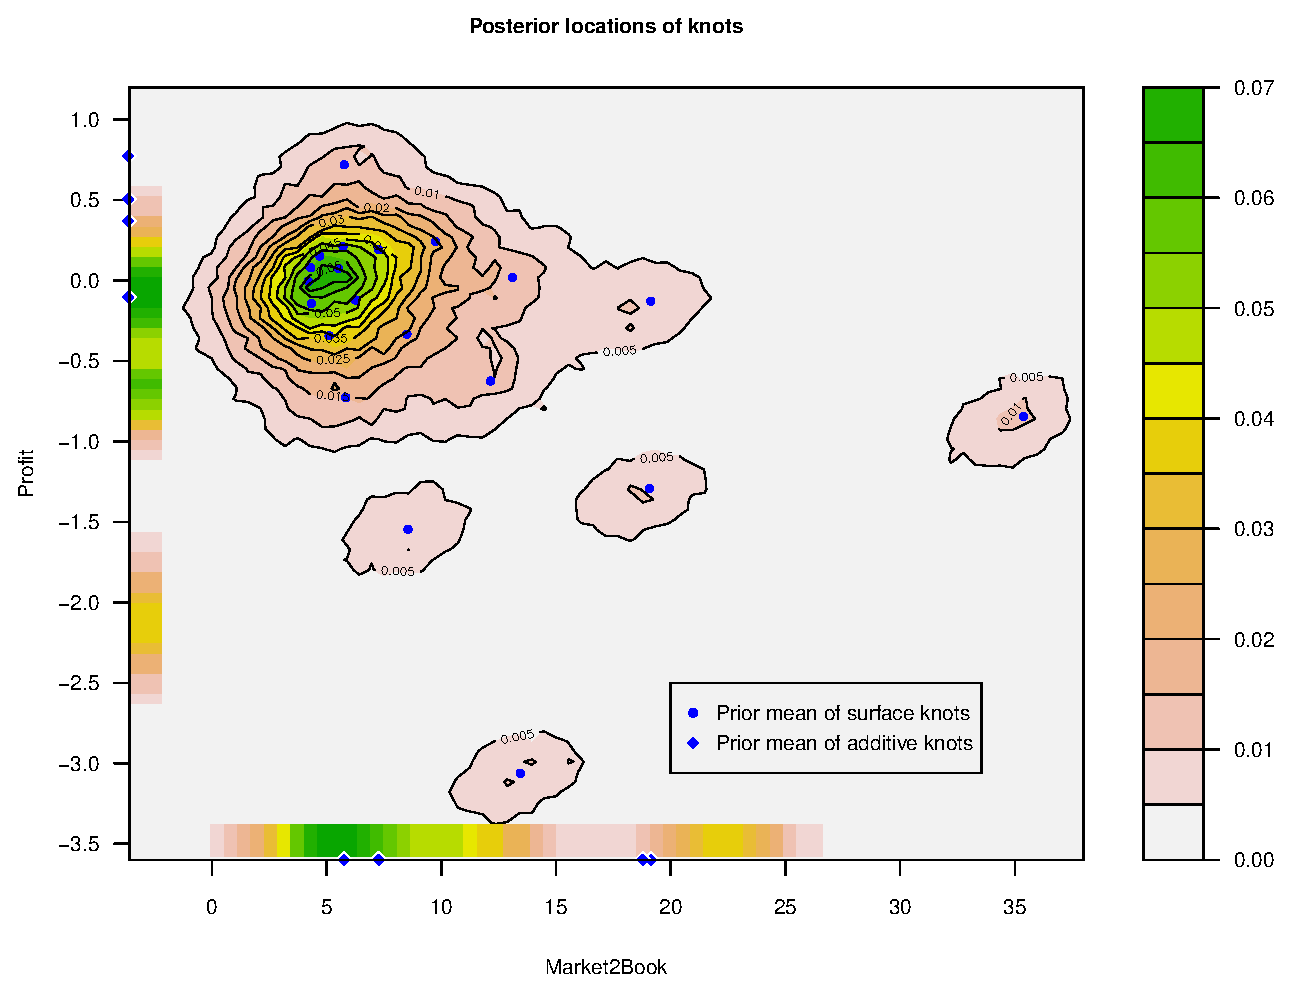
\includegraphics[height=0.8\textheight]{RajanPostKnots.eps}
    \end{figure}
  \end{center}
\end{frame}

\begin{frame}
  \frametitle{Modeling nonlinear mean with splines to firm leverage data}
  \framesubtitle{Posterior mean surface(left) and standard deviation(right)}
  \begin{center}
    \begin{figure}
      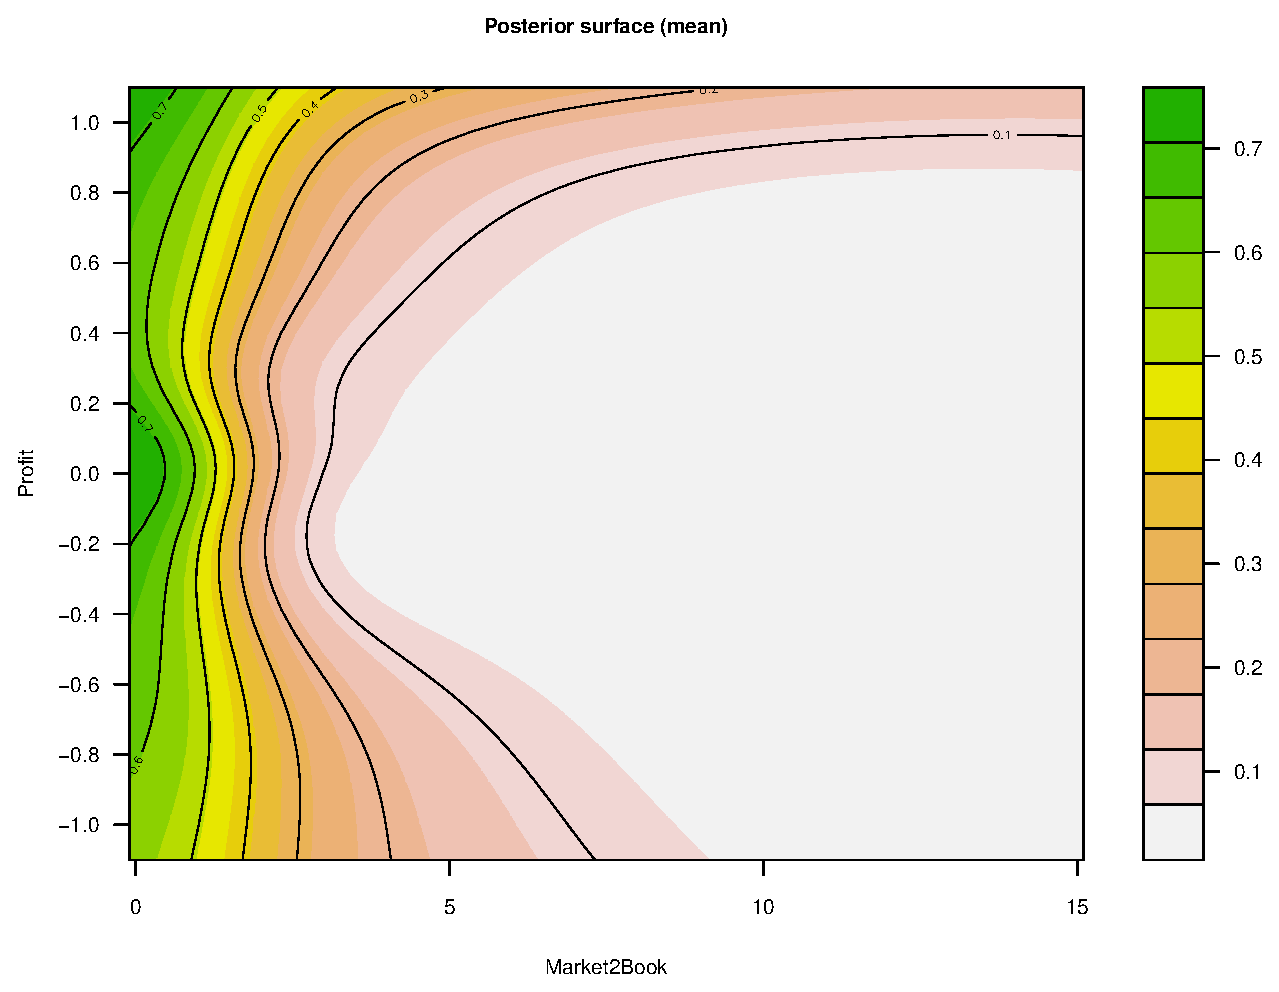
\includegraphics[width=0.5\textwidth]{RajanPostMean.eps}~~~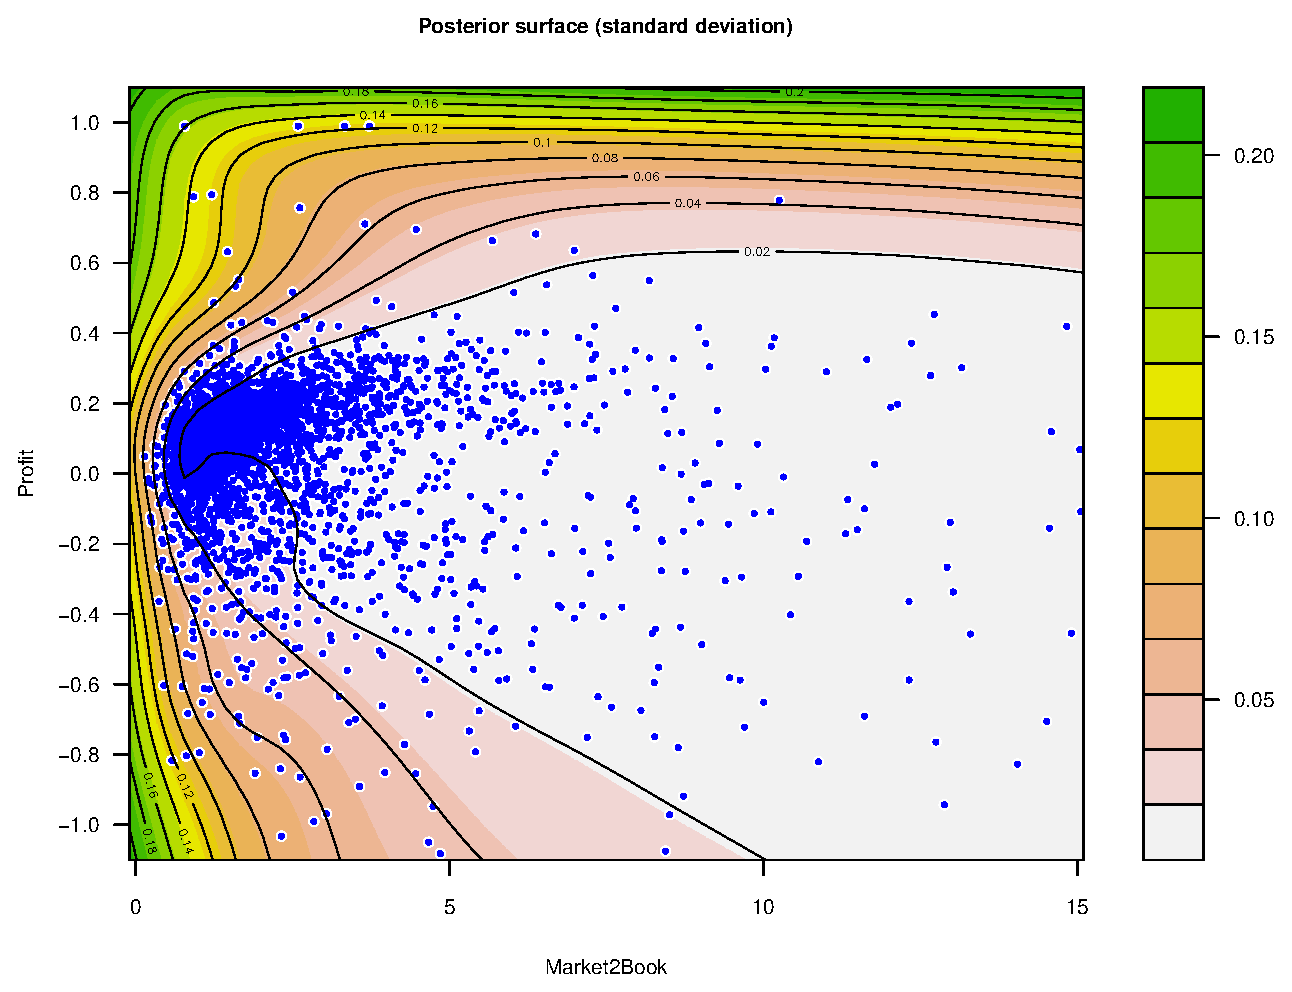
\includegraphics[width=0.5\textwidth]{RajanPostSD.eps}
    \end{figure}
  \end{center}
\end{frame}

% \section{Can we have a model that is big like an elephant?}

% \begin{frame}
%   %   \frametitle{Knowing the elephant}
%   \frametitle{Can we have a model that is big like an elephant?}

%   \begin{figure}
%     \centering
%     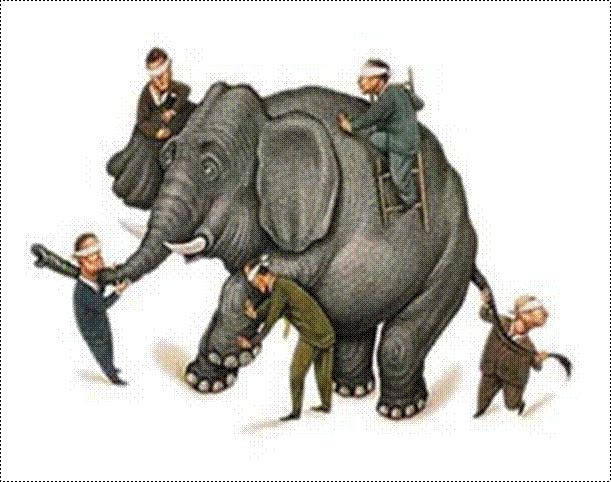
\includegraphics[height=0.8\textheight]{elephant}
%   \end{figure}
%   \tiny{by John Godfrey Saxe (1816-1887)}
% \end{frame}


% \begin{frame}
%   \frametitle{Knowing the elephant}

%   \begin{itemize}
%   \item Sophisticated models are essential for such situations.
%   \item In principle, the complicated model should be able to capture more
%     complicated data features.
%   \item Estimating such model is not easy.
%   \item There is huge space to explore.
%     \begin{itemize}
%     \item The computer is still not fast enough.
%     \item Techniques like parallel
%       computing should be used to speed up the computation.
%     \item Statistics with big data is the new challenge.
%     \end{itemize}
%   \end{itemize}
% \end{frame}

\section{Bayesian Densities Estimation for Complex data}

\begin{frame}
  \frametitle{Dependence for high-dimensional density with continuous
    and discrete margins}
  \begin{itemize}
  \item In principle, a high dimensional density can be construed via
    bivariate copulas and their margins.
    \begin{equation*}
      \label{eq:vine}
      \begin{split}
      &\prod_{k=1}^Mf_k(x_k)\times\\ &\prod_{i=1}^{M-1}\prod_{j=1}^{M-i}c_{i,i+j|1:(i-1)}(F(x_i)|x_1,...,x_{i-1},F(x_{i+j}|)x_1,...,x_{i-1})
      \end{split}
    \end{equation*}

  \item However this construction depends on the order of the margins.

  \item The reversible jump MCMC used is not efficient.

  \item Estimate high-dimensional tail-dependencies are more
    complicated.

  \end{itemize}

\end{frame}


\begin{frame}
  \frametitle{Surface maximization}

  \begin{itemize}
  \item The predictive density can be viewed as a \textbf{dynamic
      probability surface} conditional on $X$
    \begin{equation*}
      % \label{eq:predict}
      \begin{split}
      &p(Y_{(T+1):(T+p)}|Y_{1:T},X)=\\
&\prod\limits _{i=1}^{p}\int
      p(Y_{T+i}|\theta,Y_{1:(T+i-1)}, X_{T+i})p(\theta|Y_{1:(T+i-1)},X_{{1:(T+i-1)}})\mathrm{d}\theta.
      \end{split}
\end{equation*}

\item Where is the maximum point of the surface?

\begin{equation}
\label{eq:pred}
x_{best} = \mathrm{argmin}_{x} \int a (f,x) d F(x)
\end{equation}

where $a(f,x)$ is called the \textbf{acquisition function}.

\item This approach is called \textbf{Bayesian Global Optimization}.

\item Used mostly in engineering but not in statistics.

  \end{itemize}


\end{frame}

\section*{References}
\begin{frame}[allowframebreaks]
  \frametitle{References}
  \begin{small}
    % \phantomsection
    % \addcontentsline{toc}{section}{\bibname}
    \def\newblock{\hskip .11em plus .33em minus .07em} % important line
    \bibliographystyle{asa}
    \bibliography{full,References}
  \end{small}
\end{frame}


\section*{}
\begin{frame}

  \addtocounter{framenumber}{-1}

  % \emph{...essentially, all models are wrong, but some are useful}\\
  % \hfill --- George E. P. Box
  \vspace{1cm}
  \begin{center}
    {\color{SUblue} \textbf{\Huge Thank you!}}
  \end{center}

\end{frame}



\end{document}

\end{document}
